\htmlhr
\chapter{Javari immutability checker\label{javari-checker}}

Javari~\cite{TschantzE2005,QuinonezTE2008} is a Java language extension that helps programmers to avoid mutation
errors that result from unintended side effects.
If the Javari checker issues no warnings for a given program, then that
program will never change objects that should not be changed.  This
guarantee enables a programmer to detect and prevent mutation-related
errors.  (See Section~\ref{checker-guarantees} for caveats to the guarantee.)
The Javari webpage (\myurl{http://groups.csail.mit.edu/pag/javari/}) contains
papers that explain the Javari language and type system.
By contrast to those papers, the Javari checker uses an annotation-based
dialect of the Javari language.

The Javarifier tool infers Javari types for an existing program; see
Section~\ref{javari-inference}.

Also consider the IGJ checker (Chapter~\ref{igj-checker}).  The IGJ type
system is more expressive than that of Javari, and the IGJ checker is a bit
more robust.  However, IGJ lacks a type inference tool such as Javarifier.



\begin{figure}
\begin{center}
\resizebox{!}{2.5cm}{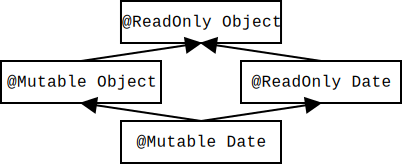
\includegraphics{figures/javari}}
\end{center}
%BEGIN LATEX
\vspace{-1.5\baselineskip}
%END LATEX
\caption{Type hierarchy for Javari's ReadOnly type qualifier.}
\label{fig:javari-hierarchy}
\end{figure}


\section{Javari annotations\label{javary-annotations}}

Five annotations are part of the Javari type system.



A programmer can write five annotations: \code{@\refclass{javari/quals}{ReadOnly}}, \code{@\refclass{javari/quals}{Mutable}},
\code{@\refclass{javari/quals}{Assignable}}, \code{@\refclass{javari/quals}{PolyRead}}, and \code{@\refclass{javari/quals}{QReadOnly}}.

\begin{description}

\item[\code{@\refclass{javari/quals}{ReadOnly}}]
  indicates a type that provides only read-only access.  A reference of
  this type may not be used to modify its referent, but aliasing references
  to that object might change it.

\item[\code{@\refclass{javari/quals}{Mutable}}]
  indicates a mutable type.
  
\item[\code{@\refclass{javari/quals}{Assignable}}]
  is a field annotation, not a type qualifier.  It indicates that the given
  field may always be assigned, no matter what the type of the reference
  used to access the field.
  
\item[\code{@\refclass{javari/quals}{QReadOnly}}]
  corresponds to Javari's ``\code{?\ readonly}'' for wildcard types.  An
  example of its use is \code{List<@QReadOnly Date>}.  It allows only the
  operations which are allowed for both readonly and mutable types.

\item[\code{@\refclass{javari/quals}{PolyRead}}]
  (previously named \code{@RoMaybe}) specifies polymorphism over
  mutability; it simulates mutability overloading.  It can be applied to
  methods and parameters.  See Section~\ref{qualifier-polymorphism} and the
  \code{@\refclass{javari/quals}{PolyRead}} Javadoc for more details.

\end{description}


\section{Writing Javari annotations\label{writing-javari-annotations}}


\subsection{Implicit qualifiers\label{javari-implicit-qualifiers}}

As described in Section~\ref{effective-qualifier}, the Javari checker
adds implicit qualifiers, reducing the number of annotations that must
appear in your code.
% For example, ...

For a complete description of all implicit Javari qualifiers, see the
Javadoc for \refclass{javari}{JavariAnnotatedTypeFactory}.


\subsection{Inference of Javari annotations\label{javari-inference}}

It can be tedious to write annotations in your code.  The Javarifier tool
(\myurl{http://groups.csail.mit.edu/pag/javari/javarifier/}) infers 
Javari types for an existing program.  It 
automatically inserts Javari annotations in your Java program or
in \code{.class} files.

This has two benefits:  it relieves the programmer of the tedium of writing
annotations (though the programmer can always refine the inferred
annotations), and it annotates libraries, permitting checking of programs
that use those libraries.



\section{What the Javari checker checks\label{javari-checks}}

The checker issues an error whenever mutation happens through a readonly
reference, when fields of a readonly reference which are not explicitly
marked with \code{@\refclass{javari/quals}{Assignable}} are reassigned, or
when a readonly expression is assigned to a mutable variable.  The checker
also emits a warning when casts increase the mutability access of a
reference.

% There is no Javadoc as of 2/2009.
% For a complete description of all checks performed by
% the Nullness checker, see the Javadoc for
% \refclass{javari}{JavariVisitor}.


\section{Examples\label{javari-examples}}

To try the Javari checker on a source file that uses the Javari
qualifier, use the following command (where \code{javac} is the JSR 308
compiler  that
is distributed with the Checker Framework).  Alternately, you may
specify just one of the test files.

\begin{Verbatim}
  javac -processor checkers.javari.JavariChecker tests/javari/*.java
\end{Verbatim}

\noindent
The compiler should issue the errors and warnings (if any) specified in the
\code{.out} files with same name.

To run the test suite for the Javari checker, use \code{ant javari-tests}.

The Javari checker itself is also annotated with Javari annotations.


% LocalWords:  PolyRead javari cp plugin ReadOnly QReadOnly romaybe Javarifier
% LocalWords:  readonly wildcard Javadoc javac RoMaybe quals IGJ
% LocalWords:  JavariAnnotatedTypeFactory
